\documentclass[11pt, spanish, a4paper, twoside]{article}

% Versión 1.er cuat 2021 Víctor Bettachini < vbettachini@unlam.edu.ar >

\usepackage[T1]{fontenc}
\usepackage[utf8]{inputenc}

\usepackage[spanish, es-tabla]{babel}
% \def\spanishoptions{argentina} % Was macht dass?
% \usepackage{babelbib}
% \selectbiblanguage{spanish}
% \addto\shorthandsspanish{\spanishdeactivate{~<>}}


\usepackage{graphicx}
\graphicspath{{./figuras/}{../LaTeX/}{../figurasLaTeX/}}
% \usepackage{float}

\usepackage[arrowdel]{physics}
\newcommand{\pvec}[1]{\vec{#1}\mkern2mu\vphantom{#1}}
% \usepackage{units}
\usepackage[separate-uncertainty= true, multi-part-units= single, range-units= single, range-phrase= {~a~}, locale= FR]{siunitx}
\usepackage{isotope} % $\isotope[A][Z]{X}\to\isotope[A-4][Z-2]{Y}+\isotope[4][2]{\alpha}

\usepackage{tasks}
\usepackage[inline]{enumitem}
% \usepackage{enumerate}

\usepackage{hyperref}

% \usepackage{amsmath}
% \usepackage{amstext}
% \usepackage{amssymb}

\usepackage{tikz}
\usepackage{tikz-3dplot}
\usepackage{tikz-dimline}
\usetikzlibrary{calc}
% \usetikzlibrary{math}
\usetikzlibrary{arrows.meta}
\usetikzlibrary{snakes}
\usetikzlibrary{decorations}
\usetikzlibrary{decorations.pathmorphing}
\usetikzlibrary{patterns}

\usepackage[hmargin=1cm,vmargin=3cm, top= 0.75cm,nohead]{geometry}

\usepackage{lastpage}
\usepackage{fancyhdr}
\pagestyle{fancyplain}
\fancyhf{}
\setlength\headheight{28.7pt} 
\fancyhead[LE, LO]{\textbf{Mecánica Analítica Computacional} }
% \fancyhead[LE, LO]{\textbf{Mecánica General} }
\fancyhead[RE, RO]{\href{https://ingenieria.unlam.edu.ar/}{$\vcenter{\hbox{
\includegraphics[height=1cm]{ambos.pdf}}}$}}
\fancyfoot{\href{https://creativecommons.org/licenses/by-nc-sa/4.0/deed.es_ES}{$\vcenter{\hbox{
\includegraphics[height=0.4cm]{by-nc-sa_80x15.pdf}}}$} \href{https://ingenieria.unlam.edu.ar/}{DIIT - UNLaM}}
\fancyfoot[C]{ {\tiny Actualizado al \today} }
\fancyfoot[RO, LE]{Pág. \thepage/\pageref{LastPage}}
\renewcommand{\headrulewidth}{0pt}
\renewcommand{\footrulewidth}{0pt}


\begin{document}
\begin{center}
  % \textsc{\large Mecánica general}\\
  \textsc{\large Cuerpo rígido | Tensores de inercia}
\end{center}

% De poder resolver estos problemas en forma autónoma puede asumir que adquirió los conocimientos mínimos sobre los temas abordados en la semana. No dude en consultar a docentes y compañeros si no puede terminarlos.
% Los problemas marcados con (*) son opcionales.

\begin{enumerate}

% \vspace{-.5cm}
% \section*{Tensores de inercia}


	\item
	\textbf{Componentes del tensor de inercia para una barra}\\
	Se tiene una barra de \(m= \SI{1}{\kilo\gram}\) de sección despreciable frente a \(l= \SI{1}{\metre}\).
	De alinear un eje (\(\hat{z}\)) con ella, 
	\begin{tasks}(2)
		\task	¿cuales son sus momentos de inercia?,
		\task ¿existen los productos de inercia? 
	\end{tasks}


	\item
	\textbf{Ejes conveniente para el cálculo del momentos de inercia}\\
	Se dibujan vistas en perspectiva de diversos objetos.
	Sabre estos dibuje los ejes intersectando en el punto más conveniente para el cálculo de momentos de inercia, esto es, en el centro de masa.
	Haga lo mismo con los dos ejes que corresponden a la proyección en planta.
	\vspace{-0.8cm}
	\begin{tasks}(4)
		\task 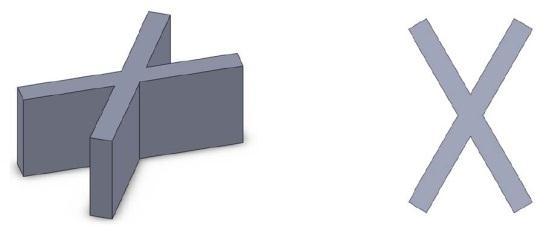
\includegraphics[width=0.15\textwidth]{o-000}
		\task 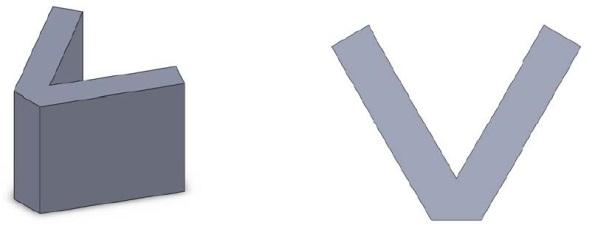
\includegraphics[width=0.15\textwidth]{o-001}
		\task 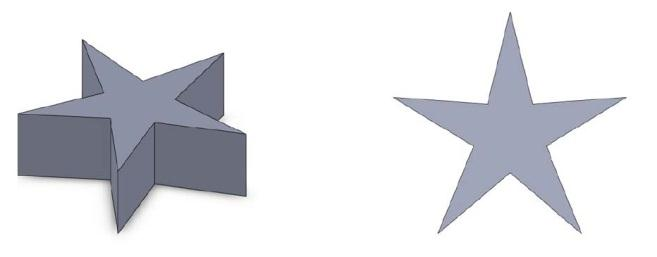
\includegraphics[width=0.15\textwidth]{o-002}
		\task 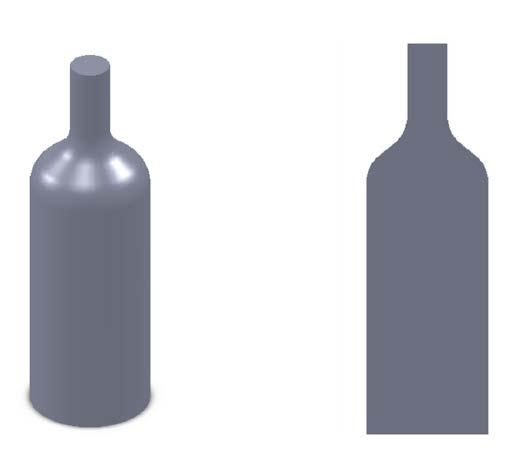
\includegraphics[width=0.15\textwidth]{o-003}
	\end{tasks}



	\item 
	\begin{minipage}[t][5.5cm]{0.65\textwidth}
		\textbf{Péndulo de torsión desbalanceado}\\
		El sistema que se muestra en la ilustración para \(t=0\) presenta pesos en los extremos de dos brazos.
		La barra dispuesta verticalmente se mantiene en tal dirección con rulemanes que posibilitan que el eje rote sin fricción con velocidad angular $\Omega$ constante respecto el marco inercial $O_{xyz}$.
		Para este análisis la masa de brazos y ejes es despreciable frente a la de los pesos \(m\).
		Calcule: 
		\begin{tasks} 
			\task tensor de inercia respecto a A en función del tiempo \(\overline{\overline{I}}_A(t)\)\\
			\task momento angular $\vec{L}_A (t) = \overline{\overline{I}}_A (t) \vec{\Omega}$ y torque $\vec{\tau} (t) = \dot{\vec{L}} (t)$.
		\end{tasks}
	\end{minipage}
	\begin{minipage}[c][0cm][t]{0.3\textwidth}
		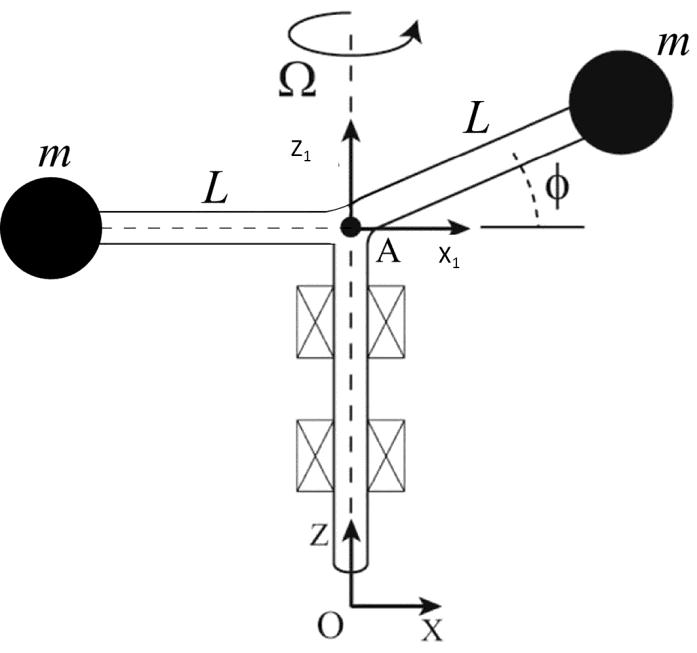
\includegraphics[width=\textwidth]{o-021}
	\end{minipage}
	Respuestas:\\
			\[
				\scalebox{0.8}{$
				\overline{\overline{I}}_A = \left[\begin{matrix}\ell^{2} m \left(- \cos^{2}{\left(\phi \right)} \cos^{2}{\left(\Omega t \right)} - \cos^{2}{\left(\Omega t \right)} + 2\right) & - \ell^{2} m \left(\cos^{2}{\left(\phi \right)} + 1\right) \sin{\left(\Omega t \right)} \cos{\left(\Omega t \right)} & \frac{\ell^{2} m \left(\sin{\left(\Omega t - 2 \phi \right)} - \sin{\left(\Omega t + 2 \phi \right)}\right)}{4}\\- \ell^{2} m \left(\cos^{2}{\left(\phi \right)} + 1\right) \sin{\left(\Omega t \right)} \cos{\left(\Omega t \right)} & \ell^{2} m \left(\sin^{2}{\left(\phi \right)} \sin^{2}{\left(\Omega t \right)} - 2 \sin^{2}{\left(\Omega t \right)} + 2\right) & - \frac{\ell^{2} m \left(\cos{\left(\Omega t - 2 \phi \right)} - \cos{\left(\Omega t + 2 \phi \right)}\right)}{4}\\\ell^{2} m \left(\cos^{2}{\left(\phi \right)} + 1\right) & - \frac{\ell^{2} m \left(\cos{\left(\Omega t - 2 \phi \right)} - \cos{\left(\Omega t + 2 \phi \right)}\right)}{4} & \ell^{2} m \left(\cos^{2}{\left(\phi \right)} + 1\right)\end{matrix}\right]
				$}
				\] 
			\[
				\vec{L}_A = \left[\begin{matrix}\frac{\Omega \ell^{2} m \left(\sin{\left(\Omega t - 2 \phi \right)} - \sin{\left(\Omega t + 2 \phi \right)}\right)}{4}\\- \frac{\Omega \ell^{2} m \left(\cos{\left(\Omega t - 2 \phi \right)} - \cos{\left(\Omega t + 2 \phi \right)}\right)}{4}\\\Omega \ell^{2} m \left(\cos^{2}{\left(\phi \right)} + 1\right)\end{matrix}\right]
			\qquad
				\vec{\tau}_A = \left[\begin{matrix}\frac{\Omega^{2} \ell^{2} m \left(\cos{\left(\Omega t - 2 \phi \right)} - \cos{\left(\Omega t + 2 \phi \right)}\right)}{4}\\\frac{\Omega^{2} \ell^{2} m \left(\sin{\left(\Omega t - 2 \phi \right)} - \sin{\left(\Omega t + 2 \phi \right)}\right)}{4}\\0\end{matrix}\right]
			\]

	\item 
	\begin{minipage}[t][2.8cm]{0.75\textwidth}
		\textbf{Molécula de agua}\\
		Calcule los momentos de inercia en el SI para una molécula de \isotope{H_2O}.
		En CNPT se abre con un ángulo de \ang{104,5;;} y median \SI{95.84}{\pico\metre} entre \isotope{O} y \isotope{H}.
		Respuesta:\\
		\[
			\scalebox{0.8}{$
			\overline{\overline{I}} = \left[\begin{matrix}1.02353565118967 \cdot 10^{-47} & 0 & 0\\0 & 1.92240664746526 \cdot 10^{-47} & 0\\0 & 0 & 2.94594229865493 \cdot 10^{-47}\end{matrix}\right]
			$}	
		\]
	\end{minipage}
	\begin{minipage}[c][2cm][t]{0.2\textwidth}
		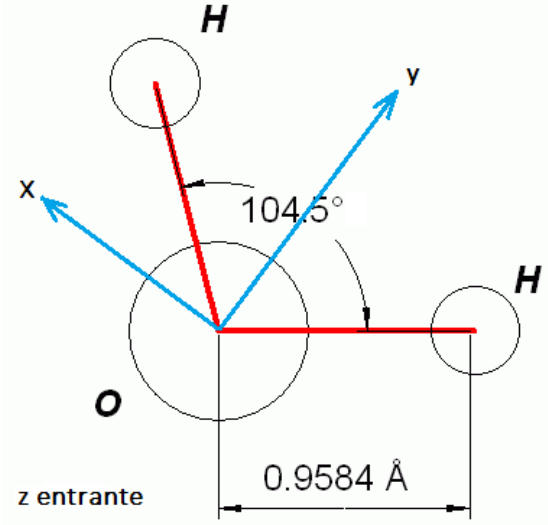
\includegraphics[width=\textwidth]{moleculaH2O}
	\end{minipage}



	\item 
	\begin{minipage}[t][4.5cm]{0.55\textwidth}
		% \begin{minipage}[t][3.5cm]{0.7\textwidth}
		% Tensor de inercia de un cubo con arista \(b\).
			\textbf{Cubo con arista \(b\)} [Marion (e) ex. 11-3]
			\begin{enumerate}
				\item Calcule el tensor de inercia desde el sistema de ejes \(x_i\) con origen en el centro de masa \(O\).
				\item Use la forma general del teorema de ejes paralelos de Steiner para calcularlo en el sistema \(X_i\) con origen en el vértice \(Q\) 
			\end{enumerate}
		\end{minipage}
		\begin{minipage}[c][2.5cm][t]{0.4\textwidth}
			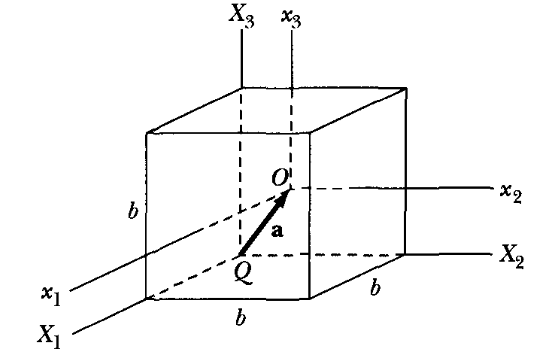
\includegraphics[width=\textwidth]{mFig11-8}
		\end{minipage}


	\item 
		\begin{minipage}[t][4cm]{0.5\textwidth}
			\textbf{Planchuela metálica calada}\\
			En una planchuela metálica homogénea se calaron dos aberturas en forma simétrica.
			Suspendida desde el punto A \emph{pendulea} en el plano \(x,y\).
			Por eso es relevante conocer su momento de inercia \(I_{zz}\) desde ese punto.
			Cuente con los datos disponibles en un taller: espesor $e$ del material, dimensiones del plano y una $m$ de pesada. 

			Se sugiere seguir esta secuencia:			
		\end{minipage}
		\begin{minipage}[c][2cm][t]{0.45\textwidth}
			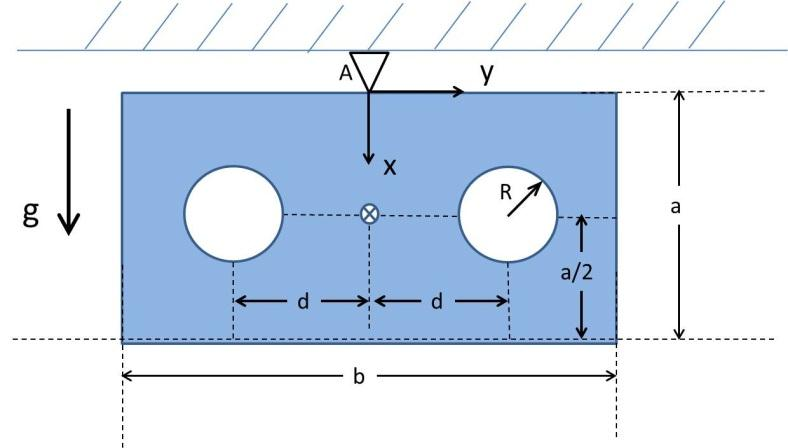
\includegraphics[width=\textwidth]{o-023}
		\end{minipage}
			\begin{enumerate}
				\item Calcular la densidad del metal de la planchuela contemplando el área faltante por los calados.
				\item Idém. \(I_{zz}\) de uno de los calados circulares como si fuera de este metal.
				\item ídem. \(I_{zz}\) de una planchuela sin calado desde su centro de masa.
				\item Trasladar con el teorema de Steiner los \(I_{zz}\) de ambos calados circulares al centro de la planchuela.
				\item Restando al \(I_{zz}\) de la planchuela sin calado el de los círculos obtenga el de la planchuela calada.
				\item Nuevamente con Steiner traslade el \(I_{zz}\) de la planchuela calada al punto de penduleo A.
			\end{enumerate}

			Respuesta:\\
			\[
			\overline{\overline{I}} = \left[\begin{matrix}\frac{m \left(6 \pi R^{4} + 24 \pi R^{2} d^{2} - a b^{3}\right)}{12 \cdot \left(2 \pi R^{2} - a b\right)} & 0 & 0\\0 & \frac{m \left(- 3 \pi R^{4} - 3 \pi R^{2} a^{2} + 2 a^{3} b\right)}{6 \left(- 2 \pi R^{2} + a b\right)} & 0\\0 & 0 & \frac{m \left(- 12 \pi R^{4} - 6 \pi R^{2} a^{2} - 24 \pi R^{2} d^{2} + 4 a^{3} b + a b^{3}\right)}{12 \left(- 2 \pi R^{2} + a b\right)}\end{matrix}\right]	
			\]


	\item 
		\begin{minipage}[t][2.3cm]{0.65\textwidth}
			\textbf{Cilindro rodando en semi-cilindro} [Landau \S 32 6]\\
			%Hallar la energía cinética de un cilindro homogéneo de radio \(a\) que rueda en el interior de una superficie cilíndrica de radio \(R\).
			Hallar la energía cinética de un cilindro homogéneo de radio \(a\) que rueda en el interior de una superficie cilíndrica de radio \(R\).

			Resultado:
			\[
				T = \frac{3 m \left(R - a\right)^{2} \dot{\phi}^{2}}{4}
			\]
		\end{minipage}
		\begin{minipage}[c][1cm][t]{0.3\textwidth}
			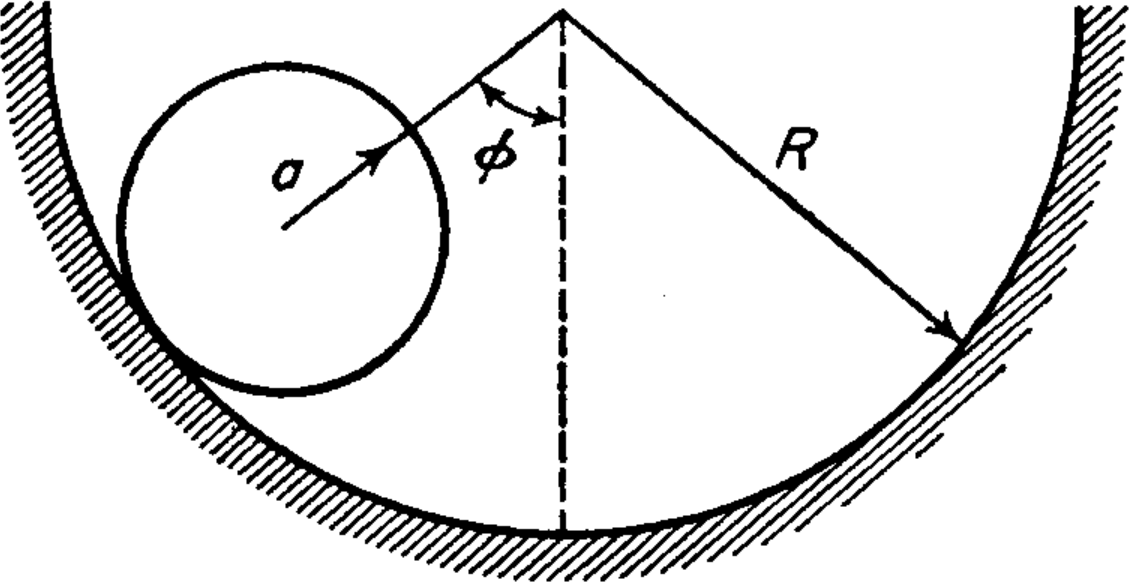
\includegraphics[width=\textwidth]{lFig41}
		\end{minipage}


	\item 
		\begin{minipage}[t][3.5cm]{0.5\textwidth}
			\textbf{Cono rodante sobre un plano} [Landau \S 32 2e y Landau \S 32 7]\\
			\begin{enumerate}
					% \item \textbf{Landau \S 32 2e} Calcule los momentos principales de inercia de un cono homogéneo de altura \(h\) y radio \(R\).
				\item En un sistema de ejes conveniente calcule el tensor de inercia de este cono homogéneo de altura \(h\) y radio en su base \(R\).
				\item Obtenga Energía cinética de dicho cono rodando sobre el plano \(X Y\).
					El contacto instantáneo \(\overline{O A}\) forma un ángulo de \(\theta\) con \(\hat{X}\).
					% \textbf{Landau \S 32 7} Hallar la energía cinética de un cono homogéneo que rueda sobre un plano.
			\end{enumerate}
		\end{minipage}
		\begin{minipage}[c][1cm][t]{0.45\textwidth}
			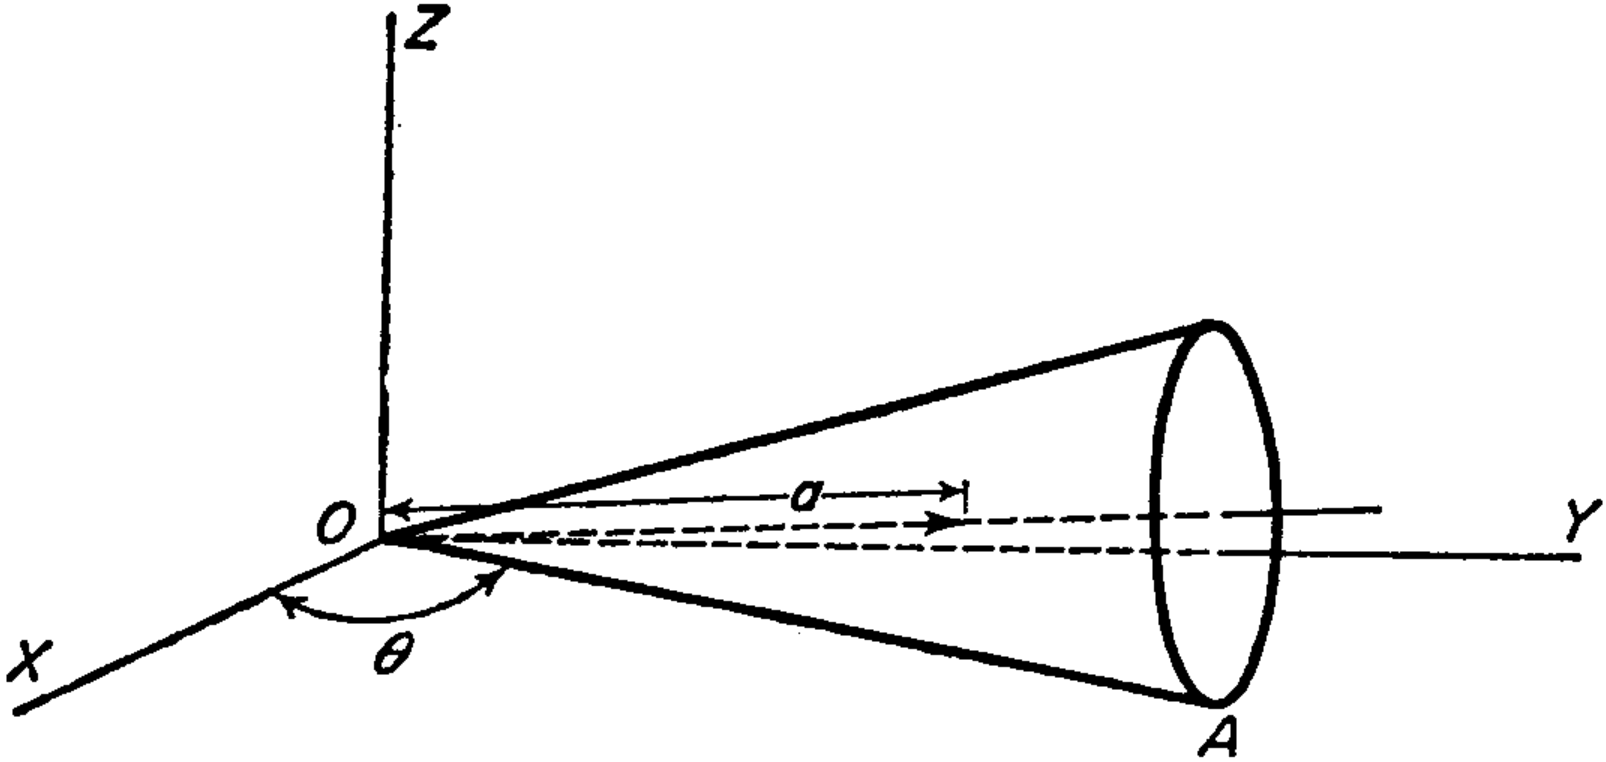
\includegraphics[width=\textwidth]{lFig42}
		\end{minipage}


\end{enumerate}

\end{document}
